%==============================================================================
% Mini Preamble.
%==============================================================================

\documentclass[11pt]{article} % 10pt article, want AMS fonts.
\makeatletter					% Make '@' accessible.
\pagestyle{myheadings}				% We do our own page headers.
\skip\footins=4ex				% Space above first footnote.
\hbadness=10000					% No "underfull hbox" messages.
\makeatother					% Make '@' special again.
\usepackage{fullpage}
\usepackage{graphicx}
\usepackage{subfigure}
%==============================================================================
% Title.
%==============================================================================

\begin{document}
\centerline{\LARGE{CSCI 2951-F Final Project}}
\centerline{Enrique and Ellis and Kavosh and Dave}
\vspace{2mm}


% --- SECTION: Paper Overview ---
\section{Paper Overview}

In this document we survey our efforts to reproduce Figures 6 and 7 from~\cite{jiang2015dependence}. The primary contribution of this paper is to relate the effectiveness of planning depth as model accuracy changes. In particular, they set out to prove, both theoretically and empirically, that with an inaccurate model, planning to a shorter depth can lead to better planning. Their Figure 6 reports results from experiments conducted by running UCT on the RockSample domain and varying the planning depth of UCT. Their Figure 7 reports results from experiments conducted by performing cross validation over possible gammas on a Randomized MDP domain.

Below, we summarize each of these domains, describe our implementation of the experiments and the hypothesize being tested, report our results from these experiments, and survey the ways in which our results and experimental setup differs from the original paper.

% --- SECTION: Domains ---
\section{Domains}

% Section: Rock Sample
\subsection{RockSample}
\label{sec: rocksample}
The RockSample domain (see Figure \ref{fig: RockSample}) consists of an agent acting in a (typically 7 $\times$ 8) GridWorld bounded by walls on the west, south and north sides. There are $k$ rocks that occupy $k$ cells of the grid world where some rocks are good and some rocks are bad. There are $5+k$ actions available to the agent, $\{North, East, South, West, Sample, Check_1 \ldots Check_k\}$. 

If the agent calls $Sample$ while it is on top of a good rock it receives $+10$ reward and if it does so while on top of a bad rock it receives $-10$ reward. The agent also receives $+10$ reward if it runs off the east edge of the GridWorld, thereby terminating the episode.

The state space is fully observable to the agent except the goodness of rocks -- that is, it always knows its own position and that of all rocks, but not the goodness of the rocks. The $Check_i$ action provides the agent with noisy knowledge of the $i$th rock. If the agent is directly on top of $rock_i$ the $Check$ action returns the true goodness of the rock. As the agent gets further and further from the rock that it is $Check$ing, the fidelity of its sensor falls off exponentially, bottoming out at a $50\%$ probability of returning the true goodness of the rock it is $Check$ing. The agent's initial belief state is that each rock has a $50\%$ chance of being good.

\begin{figure}[h]
\label{fig: RockSample}
\centering
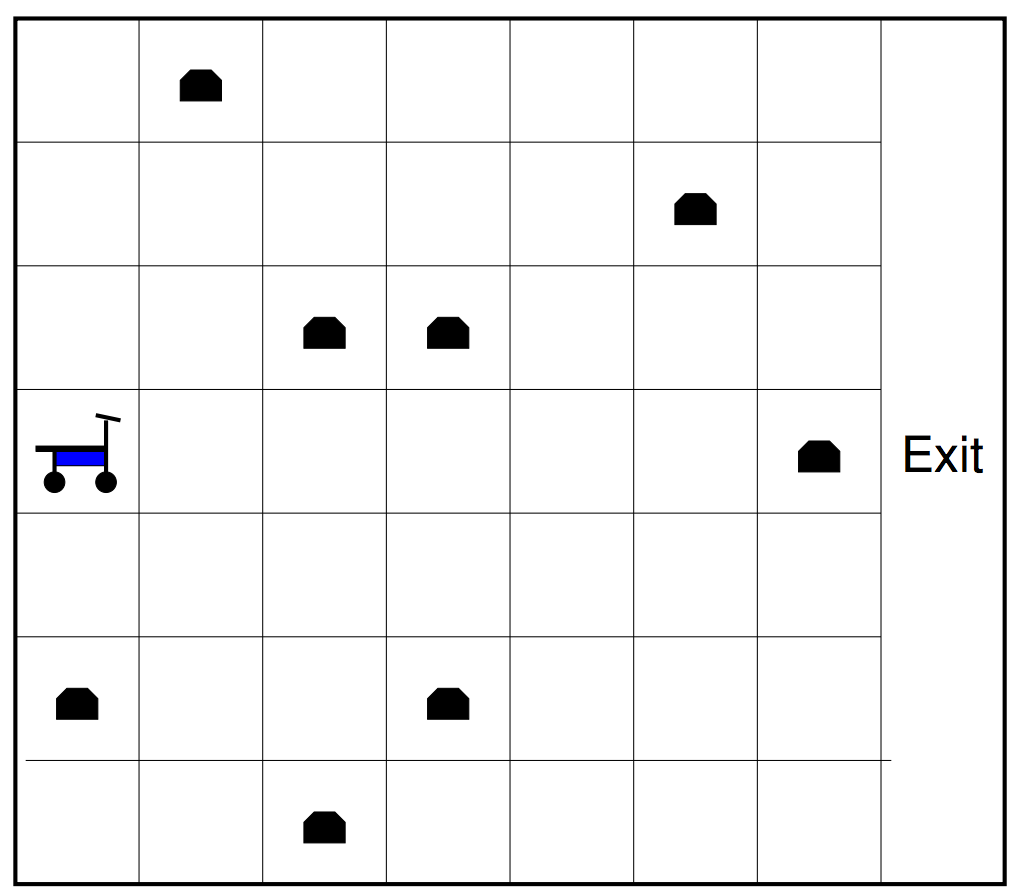
\includegraphics[page=1,width=.42\textwidth]{rock_sample_domain.png} \\
\caption{An example rock sample domain}
\end{figure}

% Section: Randomized MDPs
\subsection{Randomized MDPs}


% --- SECTION: Experiments ---
\section{Experiments}
\subsection{Figure 6}
Figure 6 of the paper tests the hypothesis that a shorter planning depth can often lead to better behavior when planning by rolling out behavior since rollout behavior induces an inaccurate model of the MDP. The rollout algorithm the authors use is Upper Confidence Bound with Trees (UCT), a Monte Carlo algorithm which uses confidence bounds in the style of Upper Confidence Bound (UCB).

The hypothesis was tested on a RockSample domain as described in Section \ref{sec: rocksample}. We implemented a RockSample domain and code to generate our plots using the Brown-UMBC (BURLAP)\footnote{http://burlap.cs.brown.edu/}.\footnote{Our code is available at https://github.com/eareyan/RLFinalProject.}

\subsection{Figure 7}

Idea: Discuss how we chose to implement our version of the experiments and the hypothesis being tested?

% --- SECTION: Results ---
\section{Results}


\subsection{UCT Performance vs. Planning Depth on Rock Sample}
Our UCT results roughly capture the same trend that those of \cite{jiang2015dependence}. The trend which we would we would hope to show is an increase in planning efficacy using an intermediate -- rather than very low or very high -- planning depth for UCT. Two of our three curves, UCT with 50 and 200 trajectories, demonstrated exactly this trend while our third curve, UCT with 1000 trajectories, performed equally well with intermediate and high planning depths. See Figure \ref{fig: UCTOurResults} for complete results. We conjecture that the discrepancies in our results are symptoms of the differences in our experimental setup -- see Section \ref{sec: repDisc} for more detail.

\begin{figure}[h]
\centering
\subfigure[Our results]{
\label{fig: UCTOurResults}
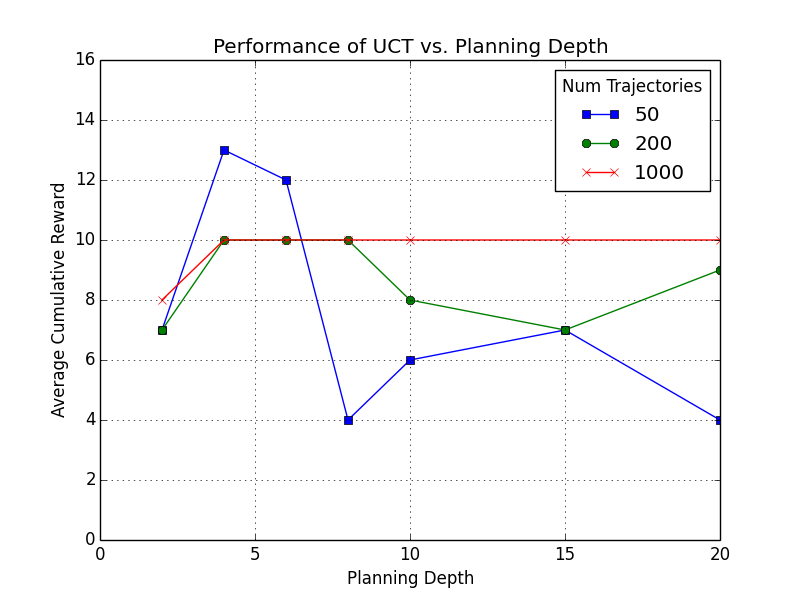
\includegraphics[page=1,width=.47\textwidth]{../results/rock_sample_results.png}}
\hspace{1mm}
\subfigure[Their results]{
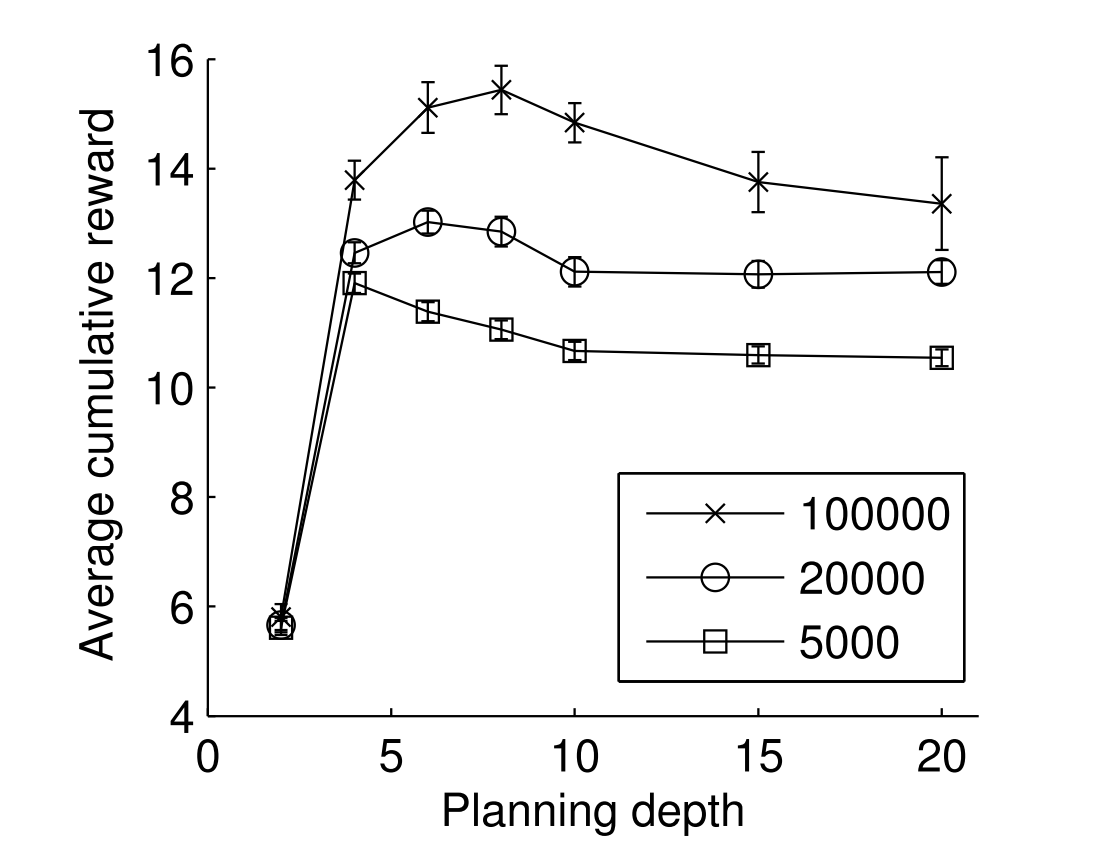
\includegraphics[page=1,width=.42\textwidth]{../results/figure_6.png}}
\caption{A comparison of our results and their results for UCT Experiments.}
\end{figure}



% Subsection: Cross validation with RandomMDP
\subsection{Cross validation with RandomMDP}

\begin{figure}
\centering
\subfigure[Our results]{
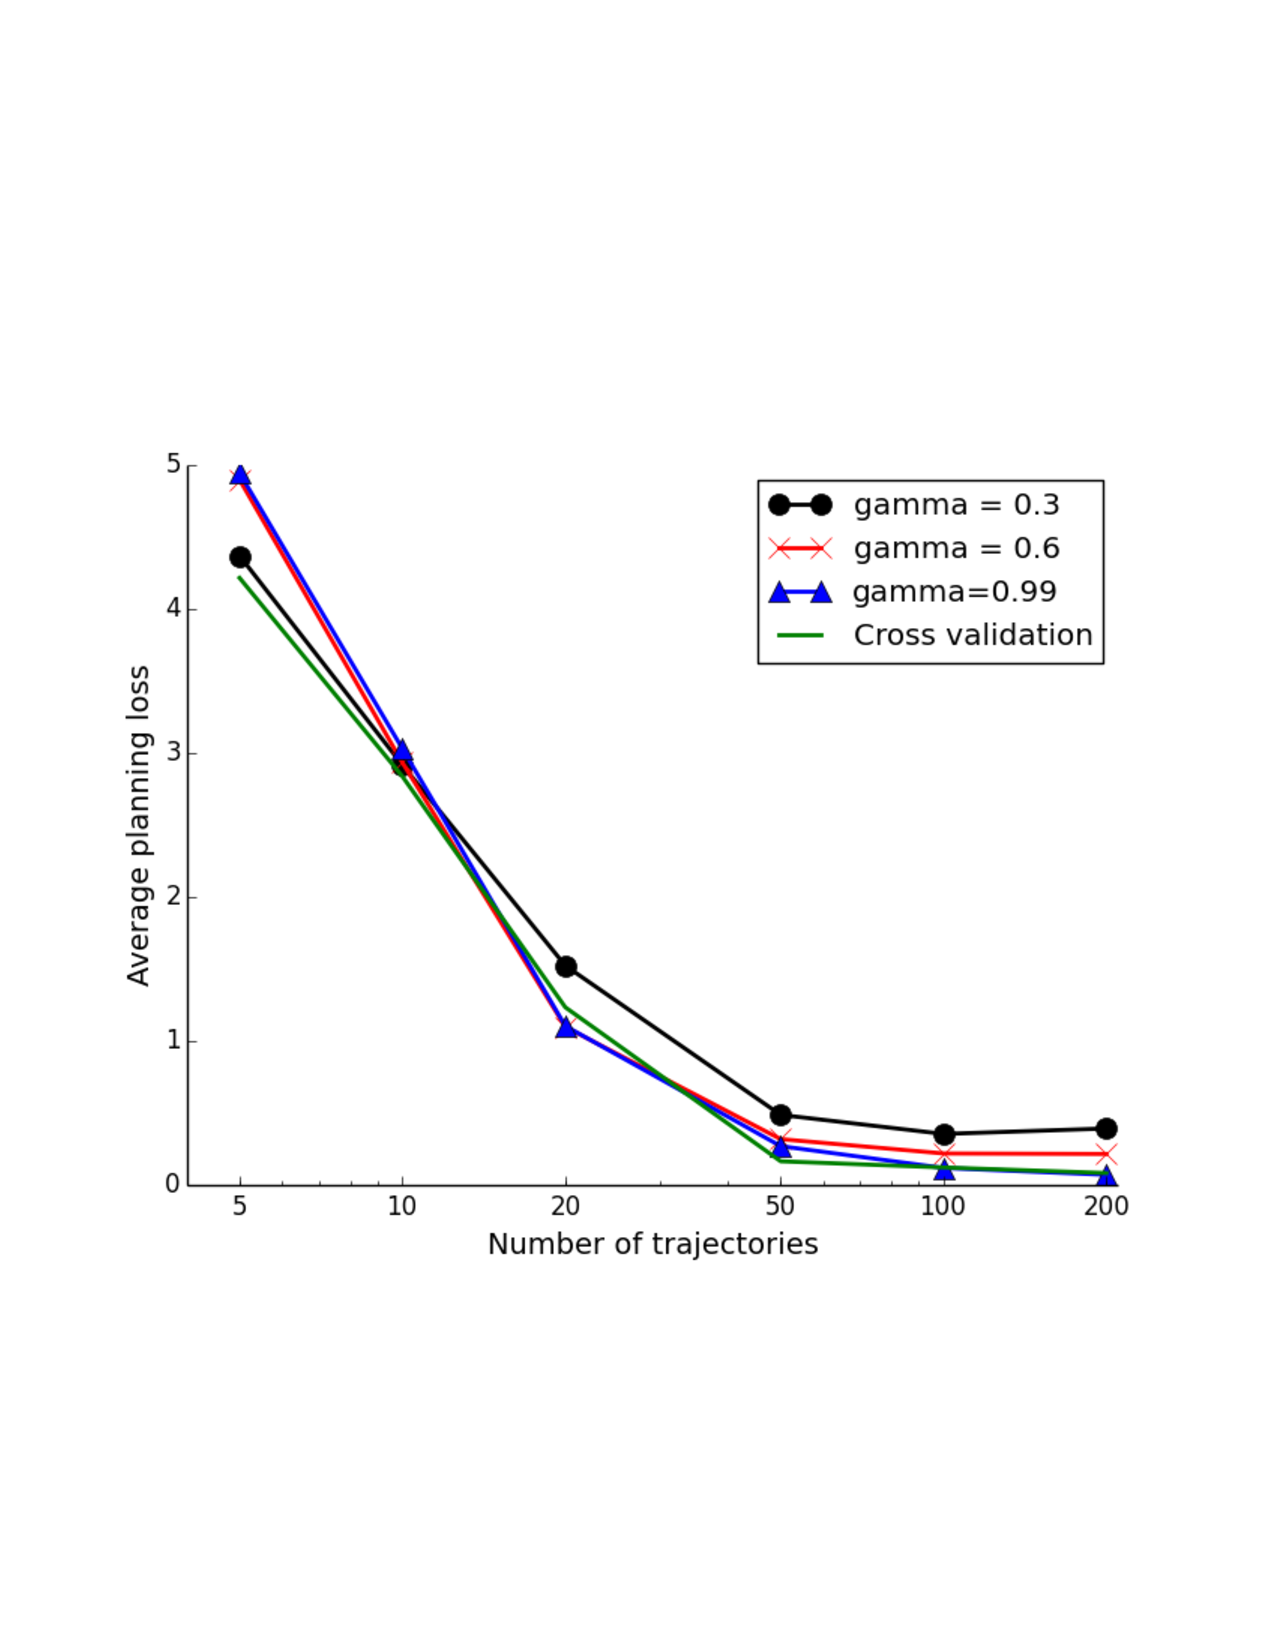
\includegraphics[page=1,width=.45\textwidth]{../results/figure_2.pdf}}
\hspace{4mm}
\subfigure[Their results]{
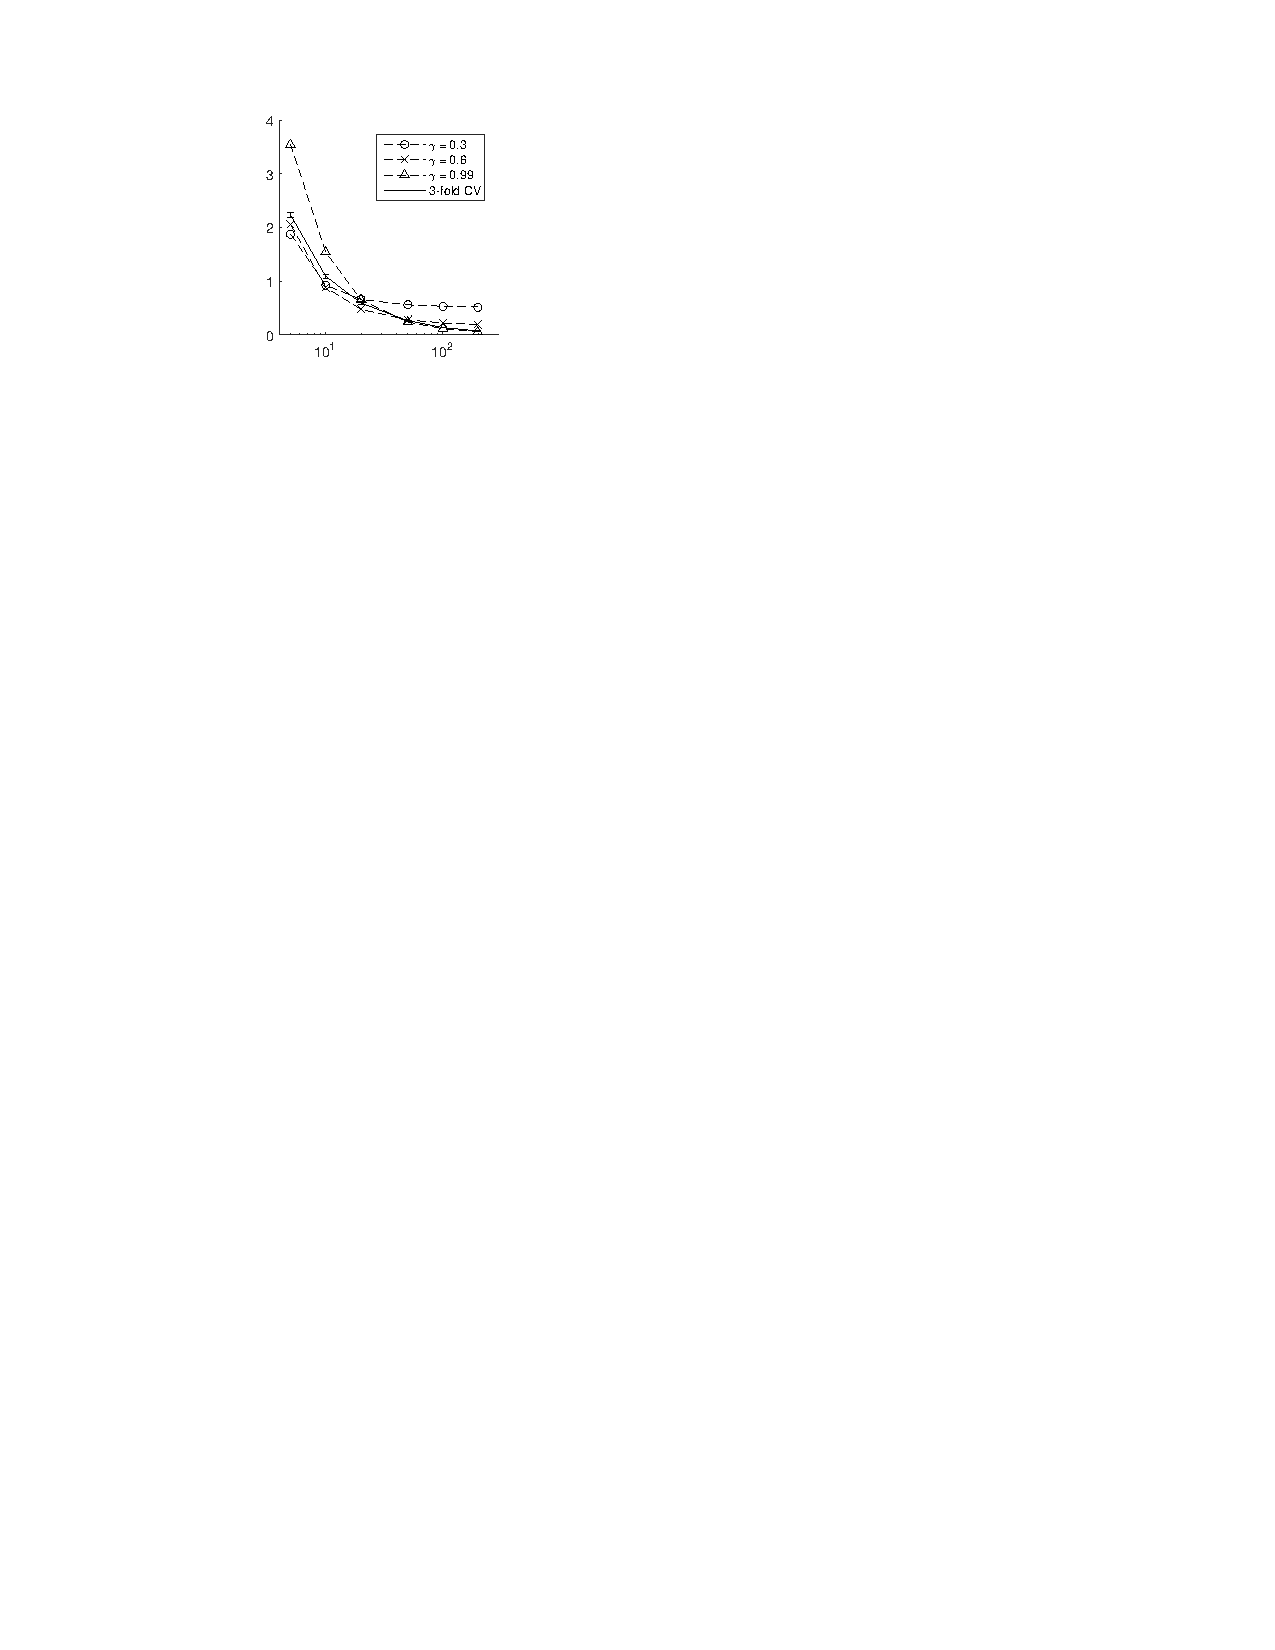
\includegraphics[page=1,width=.35\textwidth]{../results/originalCV.pdf}}
\caption{A comparison of our results and their results for Random MDP Experiments.}
\end{figure}

% --- SECTION: Reproducibility Discussion ---
\section{Reproducibility Discussion}
\label{sec: repDisc}

There were a number of ambiguities in \cite{jiang2015dependence} as well as computational constraints placed on us which prevented us from perfectly recreating the results of \cite{jiang2015dependence}. 

\subsection{Ambiguity about RockSample}
The initial state of the agent was underspecified. It was not stated whether the same initial state was used in each episode or if the state was initially randomized. In the case of the former, it was not clear what the initial state would be and in the case of the latter the distribution over states and number of rocks was indeterminate. We consulted the authors on this and were able to to determine that the same initial state with 8 rocks at fixed locations was used. However, we used only 2 rocks at fixed locations. Similarly, the initial goodness of rocks was not specified -- we assumed all rocks are initially good.

There was additional ambiguity regarding the the fidelity falloff of the $Check$ actions. We assumed the distance between the agent and a rock (which determines how unreliable the sensor is) is measured using Euclidean distance. We could have also reasonably used Manhattan distance since the agent cannot move diagonally. It was also unclear what the decay rate for exponential falloff was; we used $\frac{1}{2}$.

\subsection{Ambiguity about UCT}

Running UCT involves assigning several parameters that can dramatically alter results. For instance, the assignment of the exploration bias (i.e. the UCB parameter) will affect how UCT plans. The paper reports that they assigned this parameter for each datapoint by optimizing over the set $10 * \exp{-2, -1, 0, 1, 2}$. We fixed this parameter to be the maximum, $10 \cdot \exp(2) \approx 74$ for all experiments since we lacked the computational resources required to optimize in this way (see Section \ref{sec: compLim}).

Additionally, the value of the discount factor $\gamma$ is critical in determining behavior, especially in a domain like rock sample where there are large bursts of reward in the distance. We set $\gamma$ to be $0.9$ for our experiments, but after communicating with the authors, discovered there setting of $\gamma$ was 0.99 (although they were unsure). 

Lastly, there are several different ways one could imagine running UCT on a POMDP. We chose to convert the POMDP into a BeliefMDP and run UCT on the BeliefMDP, both during simulation and evaluation. The authors chose to sample ground states from their belief state during simulation but evaluate the performance of UCT by explicitly tracking the belief state using a generative model of the ground MDP.

\subsection{General Computational Limits in RockSample}
\label{sec: compLim}
The full barrage of experiments used by \cite{jiang2015dependence} is extremely computationally taxing. They ran ~10,000 trials per data point, with very high number of UCT trajectories and 8 rocks which leads to ~16,000 states over which belief state updates must be performed. 

We were forced to dramatically reduce the complexity of these parameters. We ran 10 trials per data point, with 100$\times$ fewer trajectories with only 2 rocks which leads to ~200 states over which belief state updates must be performed. Even after a series of optimizations for BURLAP, it still took over 5 hours to fully gather our data.


% --- BIBLIOGRAPHY ---
\bibliographystyle{acm}
\bibliography{lsdm_final}

\end{document}